% TODO proof-reading
\subsectionold{\EN{First example}\RU{Первый пример}}

\EN{Let's proceed with a simple code patching task.}
\RU{Перейдем к простой задаче модификации кода.}

\begin{lstlisting}
public class nag
{
	public static void nag_screen()
	{
		System.out.println("This program is not registered");
	};
	public static void main(String[] args) 
	{
		System.out.println("Greetings from the mega-software");
		nag_screen();
	}
}
\end{lstlisting}

\EN{How would we remove the printing of \q{This program is not registered} string?}
\RU{Как можно избавиться от печати строки \q{This program is not registered}?}

\EN{Let's load the .class file into IDA:}
\RU{Наконец загрузим .class-файл в IDA:}

\begin{figure}[H]
\centering
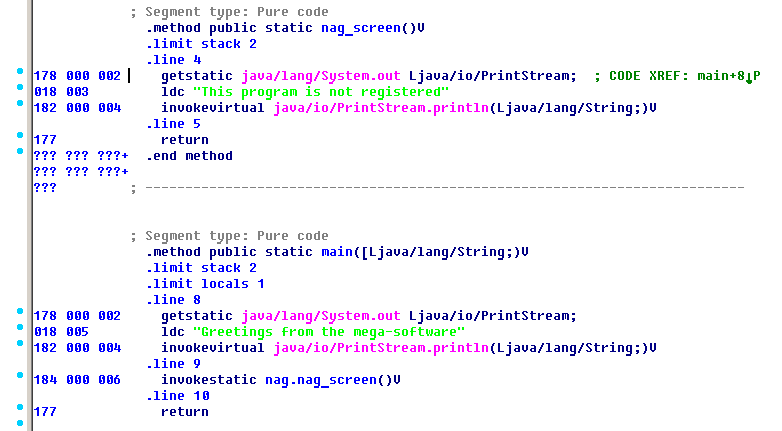
\includegraphics[scale=\FigScale]{Java_and_NET/java/13_patching/1/1.png}
\caption{IDA}
\end{figure}

\EN{Let's patch the first byte of the function to 177 (which is the \TT{return} instruction's opcode):}
\RU{В начале заменим первый байт функции на 177 (это опкод инструкции \TT{return}):}

\begin{figure}[H]
\centering
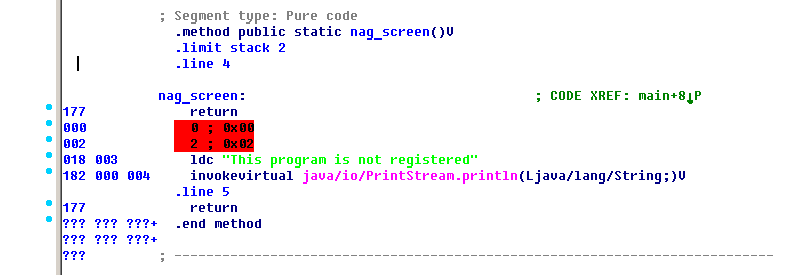
\includegraphics[scale=\FigScale]{Java_and_NET/java/13_patching/1/2.png}
\caption{IDA}
\end{figure}

\EN{But that doesn't work}\RU{Но это не работает} (JRE 1.7):

\begin{lstlisting}
Exception in thread "main" java.lang.VerifyError: Expecting a stack map frame
Exception Details:
  Location:
    nag.nag_screen()V @1: nop
  Reason:
    Error exists in the bytecode
  Bytecode:
    0000000: b100 0212 03b6 0004 b1

        at java.lang.Class.getDeclaredMethods0(Native Method)
        at java.lang.Class.privateGetDeclaredMethods(Class.java:2615)
        at java.lang.Class.getMethod0(Class.java:2856)
        at java.lang.Class.getMethod(Class.java:1668)
        at sun.launcher.LauncherHelper.getMainMethod(LauncherHelper.java:494)
        at sun.launcher.LauncherHelper.checkAndLoadMain(LauncherHelper.java:486)
\end{lstlisting}

\EN{Perhaps JVM has some other checks related to the stack maps.}%
\RU{Вероятно, в JVM есть проверки связанные с картами стека.}

\EN{OK, let's patch it differently by removing the call to \TT{nag()}:}
\RU{ОК, попробуем пропатчить её иначе, удаляя вызов функции \TT{nag()}:}

\begin{figure}[H]
\centering
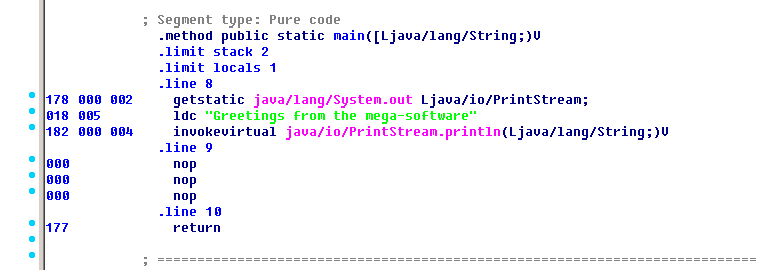
\includegraphics[scale=\FigScale]{Java_and_NET/java/13_patching/1/3.png}
\caption{IDA}
\end{figure}

\EN{0 is the opcode for \ac{NOP}.}
\RU{0 это опкод инструкции \ac{NOP}.}

\EN{Now that works}\RU{Теперь всё работает}!
